\section{Phase 2: Entwurf des Data Warehouse}

\subsection{Relationale Umsetzung eines MDM-Schemas}
\label{ref:mdmSchema}

Für die Realisierung, der in Phase 1 entworfene Data Cube wird das nachfolgende relationale Modell verwendet.
Hierbei wurde zwischen dem Star- und dem Snowflake-Schema abgewogen. 
Ein Star-Schema würde zwar die Struktur des Cubes weiter vereinfachen, aber dafür die Redundanz steigern und die Größe der Tabellen ausweiten. 
Ein Snowflake-Schema sorgt zwar für normalisierte Tabellen ohne Redundanzen, dennoch ist die Anfrageverarbeitung für solche Strukturen schwer und die Performance durch die hohe Anzahl der JOIN-Bedingungen schlechter.
Für die Umsetzung des Cubes wurde das Star-Schema ausgewählt. Hierbei gilt die Einschränkung, dass die Cube-Tabelle nur aus Foreign Keys besteht.
Diese Einschränkung hat zur Folge, dass die Dimension \texttt{PaymentSaleReturn} entstand und die Cube-Tabelle \texttt{Sales} nicht all zu groß ist. Diese Entscheidung basiert auf dem Gedanken, dass diese öfters verwendet wird und somit die Performance für die Abfragen besser ist.
Das MDM-Schema wurde somit aus Sicht der Performance und der Anfrageverarbeitung optimiert.

\begin{figure}[htbp] 
  \centering
    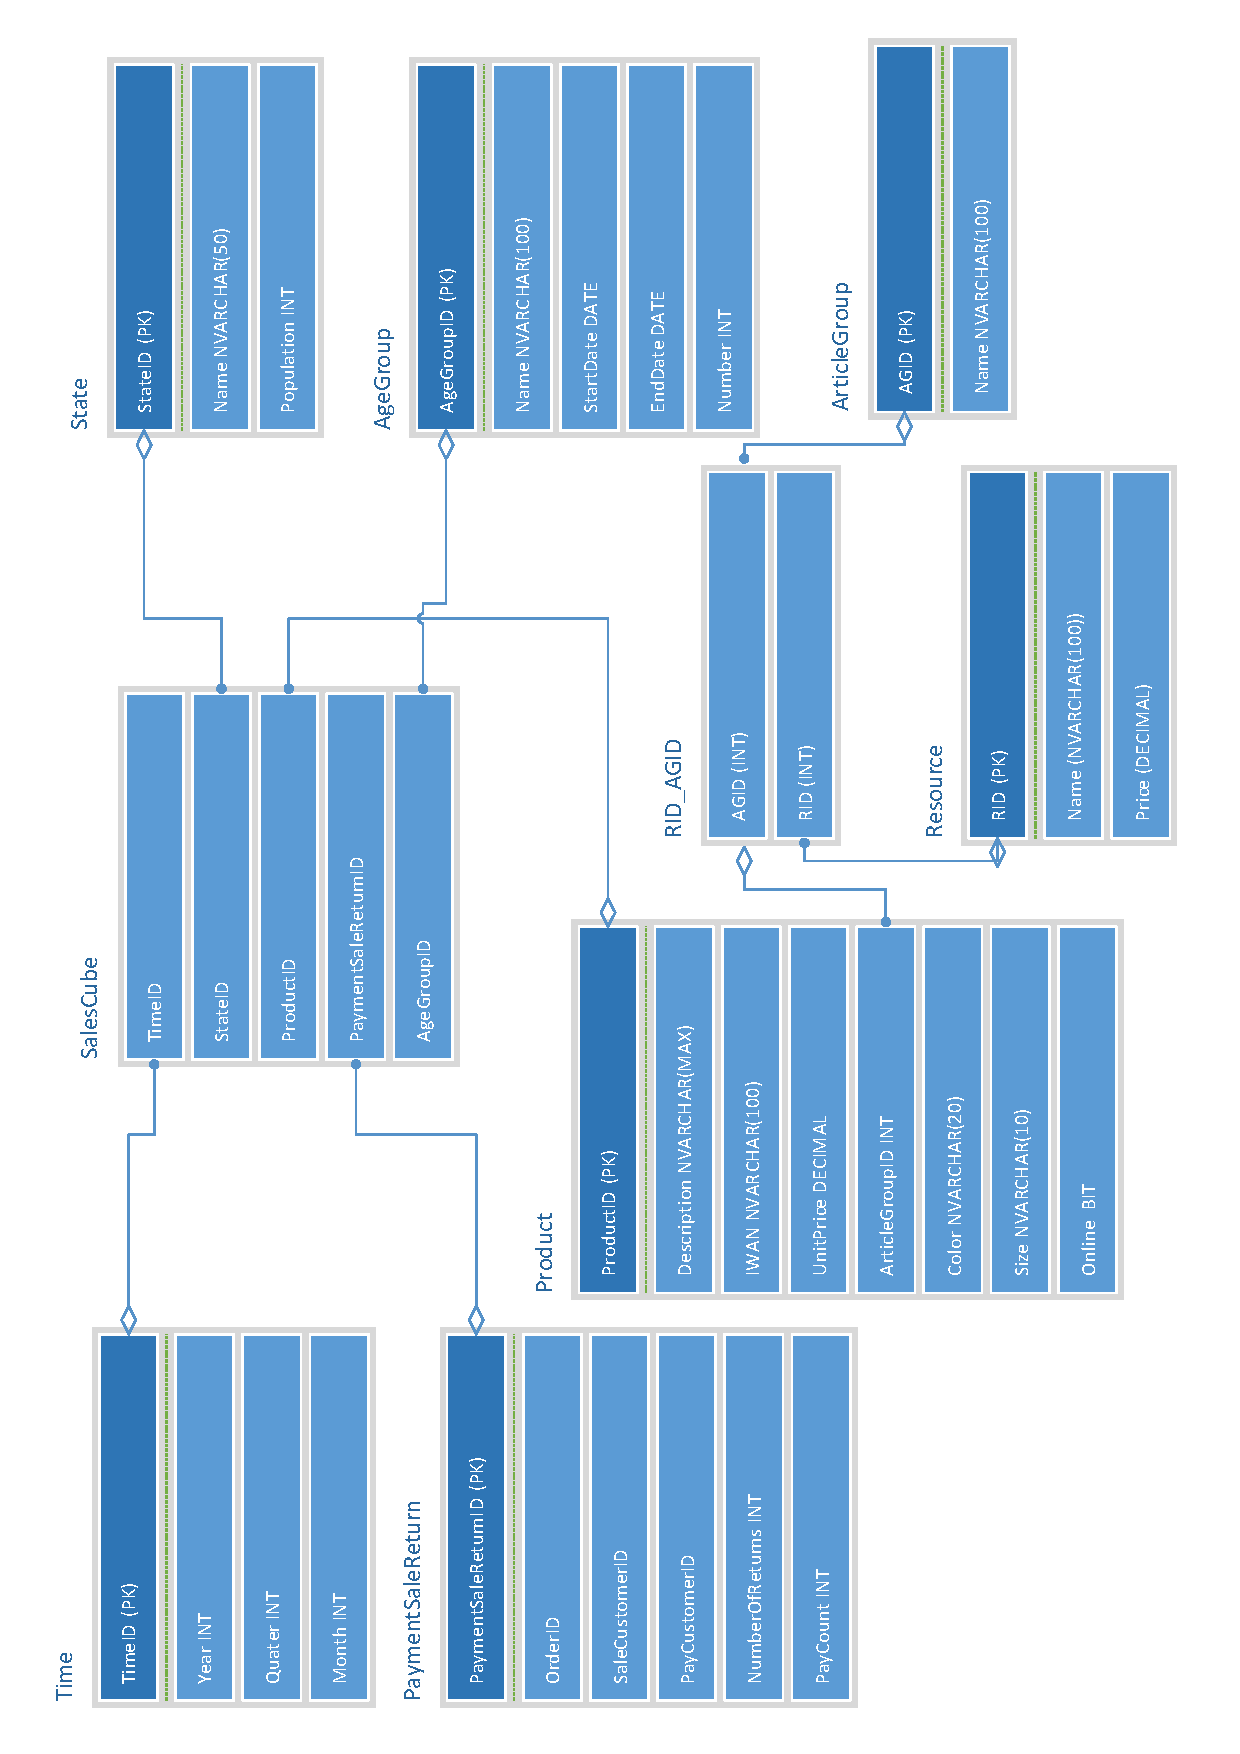
\includepdf[angle=-90,scale=0.85,offset=0.7cm -6.0cm]{phase2/SingleSchema.pdf}
    \caption{Relationales Schema des Cubes Bestellungen}
\end{figure}

\pagebreak

\subsection{Optimierung der Data Cubes}
\label{ref:optimierung}
Neben der Optimierung des Data Cubes aus Schema-Sicht (siehe \ref{ref:mdmSchema}), kann er aus Sicht der gestellten Anfragen optimiert werden.

\paragraph{Materialisierte Sichten} Eine Performance-Optimierung stellt hierbei die Nutzung von materialisierten Sichten dar, diese können sowohl für den Cube als auch für die Basis-Datenbank erstellt werden und somit den Analyse- als auch den Lade-Prozess beschleunigen. 
Für diese Sichten wäre in unserem Fall eine monatliche Aktualisierung ausreichend.

\paragraph{Index-Strukturen}Eine weitere Optimierung stellen Index-Strukturen dar. 
Der vorliegende Data Cube kann unter verschiedenen Gesichtspunkten mit Indizes angereichert werden.
Zum einen können häufig abgefragte Attribute mit kleiner Domäne mit \textbf{Bitmap-Indizes} ausgestattet werden, hierzu zählt z.B. das Attribut ''Online'' von der Tabelle Dimensionstabelle Produkt.
Außerdem können \textbf{Bitmap-JOIN-Indizes} bei \texttt{JOIN}-Partnern mit niedriger Kardinalität verwendet werden, hierzu zählen z.B. die Attribute der Ressourcen und der Artikelgruppen.
Für häufig genutzte Attribute mit großer Domäne bieten sich klassische Indexe aus den relationalen OLTP-Datenbanken wie etwa \textbf{B-Tree-Indexe} an.
Wenn multidimensionale Abfragen sehr häufig stattfinden ist es sinnvoll, multidimensionale Indexe zu verwenden wie zum Beispiel \textbf{R-Tree-Indexe}. 
Diese haben den Vorteil, dass anders als bei klassischen Indexen, nur ein einziger Index durchsucht werden muss und nicht die Ergebnisse von allen einzelnen Dimensionen zusammengeführt werden müssen.
